\documentclass[a4paper,french,10pt]{article}
\usepackage{homework}
\usepackage{diagbox}

% change le nom de la table des matières
\addto\captionsfrench{\renewcommand*\contentsname{Sommaire}}

\lstdefinelanguage{R}%
{morekeywords={function,for,in,if,elseif,else,TRUE,FALSE,%
		return, while, diag, sum, sqrt, nrow, ncol, par, plot, cbind, rep, as, survdiff, survreg, ifelse, anova,
		row, names, colnames, mean, data, frame, model, in, list, rexp, rpois, summary,
		matrix, TRUE, FALSE, for, if, else, function, NA, print, survfit, Surv, rho, ggplot},%
	sensitive=true,%
	morecomment=[l]{\#},%
	morestring=[s]{"}{"},%
	morestring=[s]{'}{'},%
}[keywords,comments,strings]%

\lstset{%
	language         = R,
	basicstyle       = \ttfamily,
	keywordstyle     = \bfseries\color{blue},
	stringstyle      = \color{magenta},
	commentstyle     = \color{olive},
	showstringspaces = false,
}

\begin{document}
	
	% Blank out the traditional title page
	\title{\vspace{-1in}} % no title name
	\author{} % no author name
	\date{} % no date listed
	\maketitle % makes this a title page
	
	% Use custom title macro instead
	\usebox{\myReportTitle}
	\vspace{1in} % spacing below title header
	
	% Assignment title
	{\centering \huge \assignmentName \par}
	{\centering \noindent\rule{4in}{0.1pt} \par}
	\vspace{0.05in}
	{\centering \courseCode~: \courseName~ \par}
	{\centering Rédigé le \pubDate\ en \LaTeX \par}
	\vspace{1in}
	
	% Table of Contents
	\tableofcontents
	\newpage
	
	%----------------------------------------------------------------------------------------
	%	EXERCICE 1
	%----------------------------------------------------------------------------------------
	

\section{Introduction}
Dans le cadre de ce projet, nous allons modéliser le comportement extrême des vagues dans le golfe du lion à l'aide des méthodes vue à travers l'unité d'enseignement HAX005X "valeurs extrêmes". D'après la source \cite{golfLion}, le golf s'étale sur 220 kilomètres de la Camargue à la frontière espagnole. La côte, essentiellement sableuse, a été façonnée par la houle (la mer gagnant souvent les terres par élévation du niveau marin) et l'érosion côtière. L'apport de sédiments en provenance des fleuves a également permis de faire avancer le rivage pendant de longues périodes. Des formations de lagunes "comme les graus" (parfois temporaires) ont pu apparaitre et ont permis de faire communiquer les étangs littoraux avec la mer. Le golf du Lion est donc un milieu naturellement dynamique. C'est dans ce contexte que nous étudions le comportement extrême des vagues à cet endroit, de façon univariée dans un premier temps puis de façon bivariée dans un second temps. 

\newpage

\section{L'algorithme EM}
Dans cette section nous allons nous intéresser à l'algorithme EM (Expectation-Maximization) afin d'estimer les paramètres $\mu$ et $\sigma$ d'un mélange gaussien. Nous avons implémenté cet algorithme via la fonction $EM$ (présente dans notre script $R$) en nous aidant de la source \cite{EM_algorithm}. Afin de tester l'efficacité de notre implémentation, nous allons dans un premier temps l'éxecuter sur des données simulées. En effet, dans notre script, nous avons implémenté une autre fonction que nous avons nommé $simulation$. Cette dernière nous permettra de générer de manière aléatoire, un échantillon issu d'un mélange gaussien. Nous décrirons plus en détaille cette fonction, en aval. Dans un second temps, nous exécuterons notre algorithme sur de vraies données afin de voir s'il est robuste. Pour cela nous utiliserons le jeu de données galaxies de la librairie MASS et nous le décrirons ultérieurement.

\subsection{Implémentation de la fonction simulation}
Comme il a été mentionné précédemment nous allons réaliser dans un premier temps une étude sur des données simulées à partir de la fonction $simulation$. Décrivons cette dernière, elle prend en argument:
\begin{itemize}
	\item \textbf{dt\_param:} Le dataframe contenant les paramètres $\alpha$, $\mu$ et $\sigma$
	\item \textbf{n:} La taille de l'échantillon
\end{itemize}
Elle retourne un vecteur de taille $n$ qui sera l'échantillon du mélange gaussien. \\ Regardons un plus en détaille comment a été conçue cette fonction. \\
La partie la plus importante et la plus subtile de ce script est celle dans laquelle nous distribuons aléatoirement les $(X_i)_{i \in 1,\dots,n}$ de l'échantillon de sorte à avoir un bon mélange gaussien. \\
Afin de simplifier les choses, rien de mieux que de prendre un exemple. Dans celui-ci, l'objectif sera de générer un mélange de quatre gaussiennes, ayant pour paramètres respectifs $\theta_1 = (\alpha_1, \mu_1, \sigma_1)$, $\theta_2 = (\alpha_2, \mu_2, \sigma_2)$, $\theta_3 = (\alpha_3, \mu_3, \sigma_3)$ et $\theta_4 = (\alpha_4, \mu_4, \sigma_4)$. \\
Les $(\alpha_j)_{j \in \{1,\dots,4\}}$ étant ici des probabilités, nous avons que:
\[
	\sum_{j=1}^{4} \alpha_{j} = 1
\]
La démarche est la suivante:
\begin{itemize}
	\item Si $Z < \alpha_1$ alors $X \sim \mathcal{N}(\mu_1, \sigma_1)$
	\item Sinon si $\alpha_1 < Z < \alpha_1 + \alpha_2$ alors $X \sim \mathcal{N}(\mu_2, \sigma_2)$
	\item Sinon si $\alpha_1 + \alpha_2 < Z < \alpha_1 + \alpha_2 + \alpha_3$ alors $X \sim \mathcal{N}(\mu_3, \sigma_3)$
	\item Sinon si $\alpha_1 + \alpha_2 + \alpha_3 < Z < \alpha_1 + \alpha_2 + \alpha_3 + \alpha_4$ alors $X \sim \mathcal{N}(\mu_4, \sigma_4)$
\end{itemize}
Notez que notre implémentation marche dans le cas général d'un mélange de J gaussiennes avec $J \in \mathbb{N}^{*}$.

\subsection{Implémentation de la fonction EM}
La fonction $EM$ est sans aucun doute celle la plus importante de cette section, il est donc primordial de la décrire. \\ 
Tout d'abord, pour implémenter cette dernière, nous nous sommes fortement aidés du pseudo-code suivant:

\begin{algorithm}
	\caption{\textbf{L’algorithme EM (Dempster et al., 1977).}}
	\begin{algorithmic}[1]
		\REQUIRE{$N \in \mathbb{N}$, $\widehat{\theta_0} \in \Theta$, un jeu de données $x_1 \dots x_n$;}
		\ENSURE
		\STATE {$k:=1$;}
		\WHILE {$K < N + 1$}
		\STATE {$\text{\textbf{ETAPE E :} \textit{Calculer la fonction }} Q(\theta;\widehat{\theta}_{k-1}) = \frac{1}{n} \sum_{i=1}^{n} \mathbb{E}_{\widehat{\theta}_{k-1}} [log f(X_i,Z_i,\theta)|X_i = x_i]$;}
		\STATE {$\text{\textbf{ETAPE M : }} \widehat{\theta}_k = argmax \hspace{1.5mm} Q(\theta;\widehat{\theta}_{k-1})$;}
		\STATE {$k \leftarrow k+1$;}
		\ENDWHILE
		\RETURN {$\widehat{\theta}_N$;}
	\end{algorithmic}
\end{algorithm}

La fonction $EM$ prend en argument:
\begin{itemize}
	\item data\_init, le dataframe contenant les paramètres initiaux ($\alpha_{init}$, $\mu_{init}$, $\sigma_{init}$)
	\item X, les données (réelles ou simulées) issues d'un mélange gaussien
	\item K le nombre d'itérations souhaitées pour l'algorithme
\end{itemize}  
Elle retourne un dataframe contenant les valeurs des
paramètres estimées par l'algorithme, à savoir $\alpha$, $\mu$ et $\sigma$. \\
Les formules que nous avons utilisé pour calculer l'étape E et M et qui sont présentées ci dessous sont issue de la source \cite{EM_algorithm}.
\begin{itemize}
	\item Lors de l'étape E nous déterminons la probabilité $\mathbb{P}_{\tilde{\theta}}(Z = j| X = X_i)$ via la formule suivante:
	\[
	\mathbb{P}_{\tilde{\theta}}(Z = j| X = X_i) = \frac{\alpha_j \times \gamma_{\mu_j, j_v}}{\sum_{k=1}^{J} \alpha_k \times \gamma_{\mu_k, v_k}}
	\] \\
	\item Lors de l'étape M, nous déterminons les estimateurs du maximum de vraisemblance $(\widehat{\alpha_j}, \widehat{\mu_j}, \widehat{\sigma_j})$ via les formules suivantes:
	\begin{align*}
		\widehat{\alpha_j} &= \displaystyle\frac{1}{n}\sum_{i=1}^n (Z=j|X=X_i) \\
		\widehat{\mu_j} &= \displaystyle\frac{\displaystyle\sum_{i=1}^n X_i (Z=j|X=X_i)}{\displaystyle\sum_{i=1}^n (Z=j|X=X_i)} \\
		\widehat{v_j} &= \displaystyle\frac{\displaystyle\sum_{i=1}^n (X_i -\widehat{\mu_j})^2 (Z=j|X=X_i)}{\displaystyle\sum_{i=1}^n (Z=j|X=X_i)}
	\end{align*} 
\end{itemize}
\vspace{7mm}
Toutefois, il est important de notifier le fait qu'il n'existe pas de convergence de la suite de paramètres établies par l'algorithme EM. En effet, ces derniers peuvent rester bloqués dans des extremas locaux. On comprend donc qu'il est primordial de choisir de bons paramètres initiaux afin de ne pas être confronté à ce problème. Dans la section consacrée à l'étude sur de vraies données, nous expliciterons la procédure qui a été mise en place pour choisir ces paramètres initiaux.

\newpage

\subsection{Étude sur des données simulées}
Cette sous-section sera consacrée à l'étude menée sur des données simulées à partir de notre fonction $simulation$.

\subsubsection{Simulation d'un mélange de deux gaussiennes } 
Nous avons ici décidé de générer un échantillon de taille 100 issu d'un mélange de deux gaussiennes de lois respectives $\mathcal{N}(\mu_1, \sigma_1) = \mathcal{N}(50, 11)$ et $\mathcal{N}(\mu_2, \sigma_2) = \mathcal{N}(220, 50)$.
La densité associée à cet échantillon a été estimée de manière non paramétrique à partir d'une méthode à noyau et elle a été tracée sur la figure \ref{density_sim}.

\begin{figure}[htp] 
	\centering
	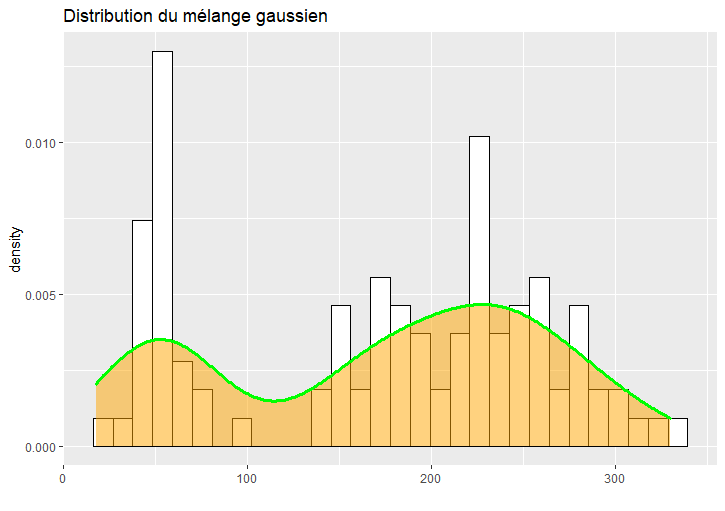
\includegraphics[scale=0.45]{images/dens_sim.png}
	\caption{Densité estimée par méthode à noyau.}
	\label{density_sim}
\end{figure}

Nous avons ensuite appliqué notre algorithme (fonction EM) sur cet échantillon. Le tableau \ref{tab1} contient les valeurs des vrais paramètres de ce mélange simulé. Comme il a été mentionné précédemment, le choix des paramètres initiaux est crucial si l'on veut que l'algorithme estime correctement les paramètres du mélange. Le tableau \ref{tab2} contient les valeurs des paramètres initiaux utilisés. Comme vous pouvez le voir en observant ces deux tableaux, nous avons choisi des paramètre initiaux assez proches des vrais de manière à ne pas être bloqué dans des extremas locaux. Les résultats obtenus par notre algorithme sont affichés sur la capture d'écran de la figure \ref{res_sim}.

 Comme on peut le voir sur la figure \ref{res_sim}, les valeurs estimées par notre implémentation sont proches de celles des vrais paramètres (voir tableau \ref{tab1}). Ces résultats nous montrent donc que notre fonction $EM$ fonctionne correctement, ce qui est rassurant.
 
 \begin{figure}[htp] 
 	\centering
 	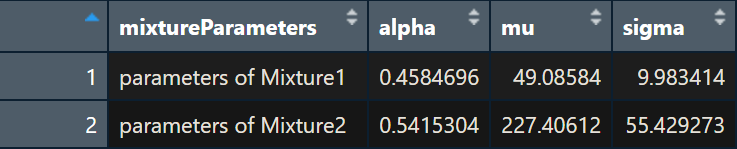
\includegraphics[scale=0.7]{images/res_sim.png}
 	\caption{Paramètres du mélange gaussien estimés par notre fonction $EM$}
 	\label{res_sim}
 \end{figure}

\begin{table}[htp]
	\center
	\begin{tabular}{|c||c|c|c|}
		\hline
		& $\alpha$ & $\mu$ & $\sigma$\\
		\hline
		Paramètres du 1er mélange & $0.4$ & $50$ & $11$ \\
		\hline
		Paramètres du 2ème mélange & $0.6$ & $220$ & $50$ \\
		\hline
	\end{tabular}
	\caption{Vrais paramètres du mélange}
	\label{tab1}
\end{table}

\newpage

\begin{table}[htp]
	\center
	\begin{tabular}{|c||c|c|c|}
		\hline
		& $\alpha_{init}$ & $\mu_{init}$ & $\sigma_{init}$\\
		\hline
		Paramètres du 1er mélange & $0.2$ & $30$ & $21$ \\
		\hline
		Paramètres du 2ème mélange & $0.8$ & $280$ & $160$ \\
		\hline
	\end{tabular}
	\caption{Paramètres estimées du mélange}
	\label{tab2}
\end{table}

\subsubsection{Simulation d'un mélange à quatre gaussiennes}
Nous avons ici décidé de générer un échantillon de taille 1000 issu d'un mélange de quatre gaussiennes de lois respectives:
\begin{itemize}
	\item $\mathcal{N}(\mu_1, \sigma_1) = \mathcal{N}(35, 11)$
	\item $\mathcal{N}(\mu_2, \sigma_2) = \mathcal{N}(350, 22)$
	\item $\mathcal{N}(\mu_3, \sigma_3) = \mathcal{N}(720, 32)$
	\item $\mathcal{N}(\mu_4, \sigma_4) = \mathcal{N}(1198, 55)$
\end{itemize}
La densité associée à cet échantillon a été estimée de manière non paramétrique à partir d'une méthode à noyau et elle a été tracée sur la figure \ref{density_sim2}.

\begin{figure}[htp] 
	\centering
	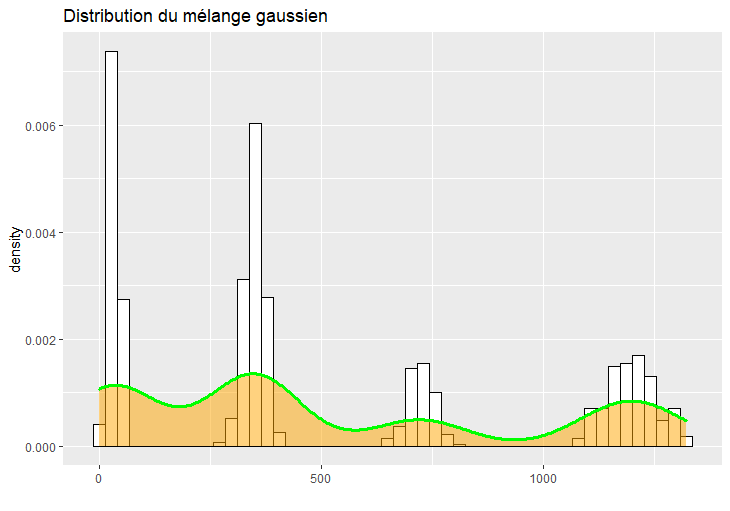
\includegraphics[scale=0.45]{images/dens_sim2.png}
	\caption{Paramètres initiaux choisis}
	\label{density_sim2}
\end{figure}

Nous avons ensuite appliqué notre algorithme (fonction EM) sur cet échantillon. Le tableau \ref{tab3} contient les valeurs des vrais paramètres de ce mélange simulé. Comme il a été mentionné précédemment, le choix des paramètres initiaux est crucial si l'on veut que l'algorithme estime correctement les paramètres du mélange. Le tableau \ref{tab4} contient les valeurs des paramètres initiaux utilisés. Comme vous pouvez le voir en observant ces deux tableaux, nous avons choisi des paramètre initiaux assez proches des vrais de manière à ne pas être bloqué dans des extremas locaux. Les résultats obtenus par notre algorithme sont affichés sur la capture d'écran de la figure \ref{res_sim2}.

Comme on peut le voir sur la figure \ref{res_sim2}, les valeurs estimées par notre implémentation sont proches de celles des vrais paramètres (voir tableau \ref{tab3}). Ces résultats nous montrent conforte une fois de plus dans l'idée que notre fonction $EM$ fonctionne correctement.

\begin{figure}[htp] 
	\centering
	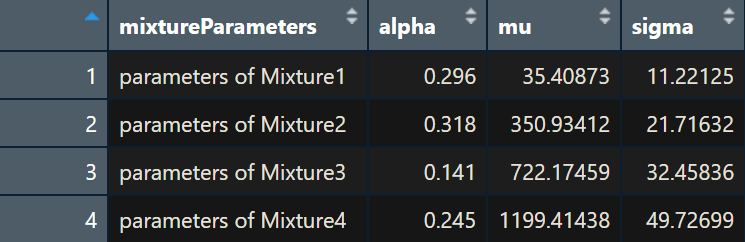
\includegraphics[scale=0.7]{images/res_sim2.png}
	\caption{Paramètres du mélange gaussien estimés par notre fonction $EM$}
	\label{res_sim2}
\end{figure}

\begin{table}[htp]
	\center
	\begin{tabular}{|c||c|c|c|}
		\hline
		& $\alpha$ & $\mu$ & $\sigma$\\
		\hline
		Paramètres du 1er mélange & $0.30$ & $35$ & $11$ \\
		\hline
		Paramètres du 2ème mélange & $0.33$ & $350$ & $22$ \\
		\hline
		Paramètres du 3ème mélange & $0.15$ & $720$ & $32$ \\
		\hline
		Paramètres du 4ème mélange & $0.22$ & $1198$ & $55$ \\
		\hline
	\end{tabular}
	\caption{Vrais paramètres du mélange}
	\label{tab3}
\end{table}

\begin{table}[htp]
	\center
	\begin{tabular}{|c||c|c|c|}
		\hline
		& $\alpha$ & $\mu$ & $\sigma$\\
		\hline
		Paramètres du 1er mélange & $0.33$ & $30$ & $10$ \\
		\hline
		Paramètres du 2ème mélange & $0.30$ & $370$ & $25$ \\
		\hline
		Paramètres du 3ème mélange & $0.17$ & $717$ & $30$ \\
		\hline
		Paramètres du 4ème mélange & $0.20$ & $1238$ & $57$ \\
		\hline
	\end{tabular}
	\caption{Paramètres initiaux choisis}
	\label{tab4}
\end{table}

%\begin{figure}[htp] 
%	\centering
%	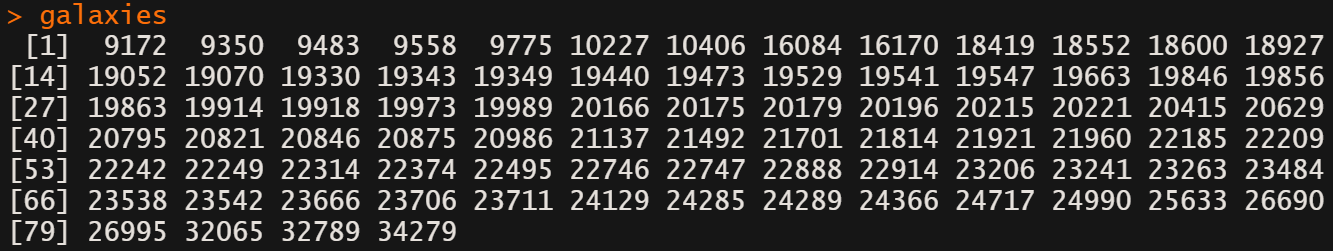
\includegraphics[scale=0.45]{images/dataset.png}
%	\caption{Extrait du jeu de données $galaxies$}
%	\label{galaxies}
%\end{figure}


\section{Comparaison de la fonction $EM$ avec $mixtools$ sur des données réelles}
Dans cette section, l'étude sera menée sur des données réelles. Nous utiliserons le jeu de données $galaxies$ provenant de la librairie $MASS$ de $R$. Dans un premier temps, nous allons estimer les paramètres du mélange associés à ce dataset via l'utilisation de notre implémentation de l'algorithme EM (la fonction EM). Nous estimerons ensuite une seconde fois les paramètres de ce même mélange mais cette fois-ci, en utilisant la fonction $normalmixEM$ prédéfinie de $R$ qui est disponible via le package $mixtools$. Nous avons choisi d'utiliser cette librairie car l'algorithme EM y est implémenté et il est utilisé par la fonction $normalmixEM$ pour estimer les paramètres d'un mélange. Le fait de comparer les résultats de notre fonction avec ceux obtenus par celle prédéfini de $R$ nous permettra d'évaluer la performance et la robustesse de notre implémentation sur de vraies données.\\
Le jeu de données $Galaxies$ est un vecteur numérique qui représente les vitesses en km/s (kilomètres par secondes) de $82$ galaxies. La figure \ref{galaxies} est un extrait de ce jeu de données.

\begin{figure}[htp] 
	\centering
	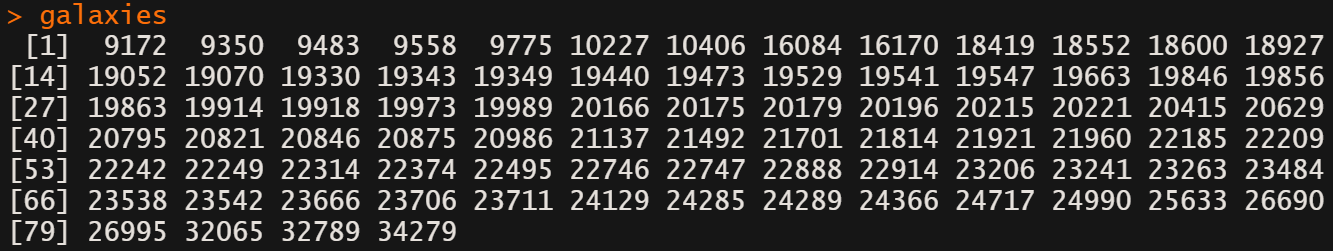
\includegraphics[scale=0.45]{images/dataset.png}
	\caption{Extrait du jeu de données $galaxies$}
	\label{galaxies}
\end{figure}

Comme il a été mentionné dans la section 2.2, si l'on veut obtenir de bonnes estimations pour les paramètres du mélange, il est primordial de sélectionner correctement les paramètres qui serviront de conditions initiales pour l'algorithme. Nous allons donc détailler la stratégie qui a été mise en place pour sélectionner ces derniers. Étant donné que nous ne connaissons pas la vraie densité associée à ces données, nous avons utilisé dans un premier temps une méthode d'estimation non paramétrique (à noyau) afin de d'estimer cette dernière. La figure \ref{realDataDensEst} représente la courbe de densité estimée par la méthode à noyau. 

\begin{figure}[htp] 
	\centering
	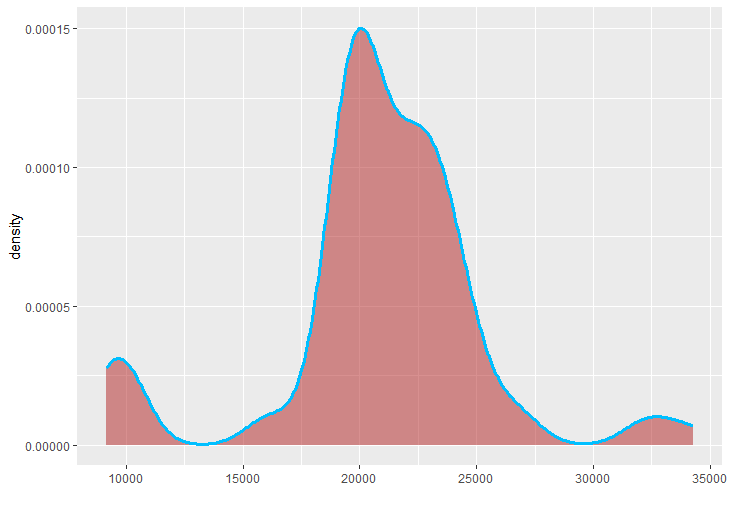
\includegraphics[scale=0.45]{images/realDataDensEst.png}
	\caption{Densité du dataset $galaxies$ estimée par une méthode à noyau}
	\label{realDataDensEst}
\end{figure}

En observant la figure \ref{realDataDensEst}, on peut facilement distinguer 3 pics principaux. Un premier vers 9800 sur l'axe des abscisses, un deuxième vers 21000 et un 3ème vers 32000. Il semblerait aussi y avoir une sorte de pic vers 24000 mais celui-ci n'étant pas clairement visible nous ne le considérerons pas. On supposera donc pour la suite de l'étude que nous somme dans le cas d'un mélange à 3 composantes.

%\begin{figure}[htp] 
%	\centering
%	\subfloat[seuil $\approx 2.7$]{%
%		\includegraphics[scale=0.4]{images/sumBadth.png}%
%	}%
%	\hfill%
%	\subfloat[seuil $\approx 3.65$]{%
%		\includegraphics[scale=0.4]{images/sumGoodth.png}%
%	}%
%	\caption{Résultats donnés en sortie de la fonction \textit{fpot} pour les 2 seuils}
%	\label{summary}
%\end{figure}


%\begin{table}[htp]
%	\center
%	\begin{tabular}{|c||c|c|c|}
%		\hline
%		\diagbox{Niveau de retour}{Périodes ou Années $T$} & $T = 100$ & $T = 500$ & $T = 1000$\\
%		\hline
%		$x_{\frac{1}{T}}$ & $4.686475$ & $4.72502$ & $4.723653$ \\
%		\hline
%	\end{tabular}
%	\caption{Niveaux de retour associés aux périodes de retour $T$}
%	\label{tab3}
%\end{table}

\newpage

\section{Conclusion}
À travers ce projet, nous avons pu voir qu'au fil des années, nous serons confrontés à des valeurs extrêmes de vagues de plus en plus grandes. Cela est sans aucun doute une conséquence de la hausse des températures et en particulier de la montée du niveau des océans. Nous comprenons donc pourquoi la lutte contre le réchauffement climatique est au cœur des enjeux scientifiques actuels. D'autre part, nous avons pu constater que plus nous prendrons des mesures issues de stations proches et plus les données associées à ces dernières seront fortement corrélées. 


\newpage


\section{THEME sur des données de Vins}

Dans cette section, à l'inverse de la partie précédente, nous nous plaçons dans un cadre non aléatoire avec un modèle à composantes, les données pour l'illustration sont issues de 21 Vins de Loire, ces Vins étant d'écrient par 2 variables qualitatives (Label: Bourgueuil, Chinon, Saumur), (Sol: En1, Env2, Référence, Env4) ainsi que 29 variables quantitatives décrivent des
caractéristiques comme l’odeur, le goût des Vins. \newline
Précisement on organise les variables quantitatives suivants les blocs de thèmes suivants : odeur, arôme, goût, note de goût, plante et composition (chimique).\newline

\begin{itemize}
	\item \textit{Odeur}, qui comprend les variables \textit{Odor.Intensity.before.shaking,~Odor.Intensity,~Quality.of.odour} décrivant les caractéristiques olfactives des Vins. 
	\item \textit{Arome}, qui renvoie aux variables \textit{Aroma.quality.before.shaking,~Aroma.intensity,~Aroma.persistency,~Aroma.quality} faisant référence aux caractéristiques sensorielles des Vins telles que l'intensité, la qualité, la précence des arômes. 
	\item \textit{Goût}, comprenant les variables renvoyant au goût fuité, amère, acide ou épicé des Vins : \textit{Fruity.before.shaking,~Fruity,~Acidity,~Spice.before.shaking,~Spice,~Bitterness}
	\item \textit{Note\_goût}, renvoyant aux notes / caractéristiques gustatives des Vins, le thème comprend les variables commes l'équilibre des saveurs \textit{Balance,~Smooth,~Attack.intensity,~Intensity,~Harmony,~Typical}
	\item \textit{Plante}, ce thème correspond à des caractères de plantes utilisées dans la fermentation des Vins : \textit{Flower.before.shaking,~Visual.intensity,~Nuance,~Surface.feeling}
	\item \textit{Composition}, ce dernier theme renvoie aux compositions chimiques des fuits utilisées, telles la teneur alcool ou l'astringence : \textit{Astringency,~Alcohol,~Phenolic,~Plante,~Flower}
\end{itemize} 

\begin{figure}[htp] 
	\centering
	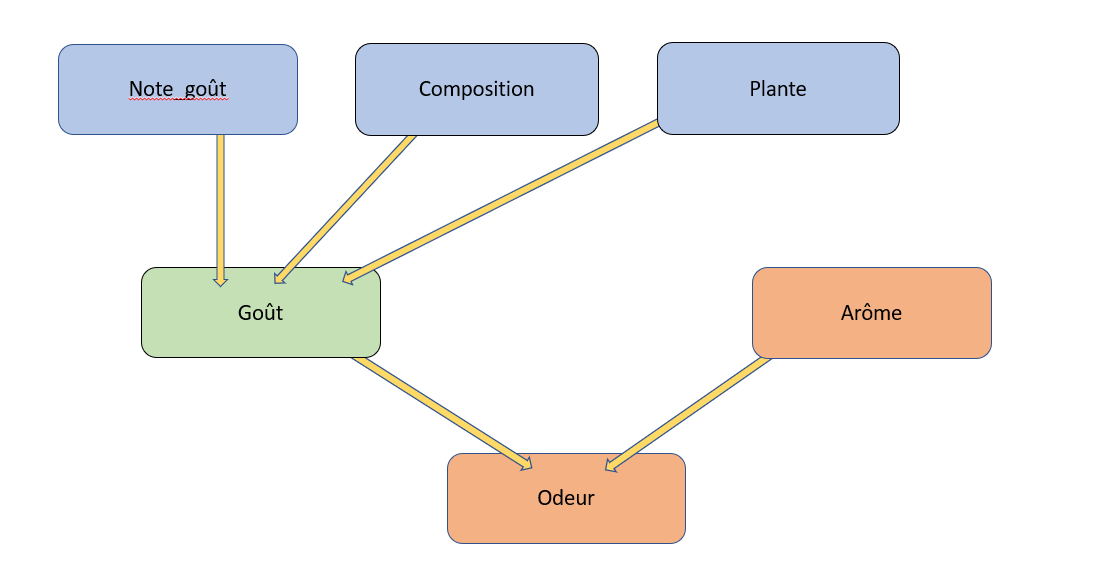
\includegraphics[scale=0.45]{images/Eq_THEME.png}
	\caption{Equations thèmatiques}
\end{figure}

On s'interresse, pour ces variables décrivant les Vins, à prédire les variables caractéristiques de l'odeur des Vins ainsi que d'en tirer des composantes explicatives. Puisque ces caractéristiques d'odeur sont à la fois liées aux variables d'arôme et de goût, elle-même dépendante des variables de composition, de note de gout et de caractéristiques de plantes utilisées dans la fermentation des Vins, l'utilisation de THEME est dans ce cas adéquate à cette recherche. Nous obtenons les deux équations thématiques suivantes : \newline

Dans un premier temps, nous avons décidé d'appliquer THEME sans \textit{cross-validation backward} en partant du modèle avec 2 composantes pour le thème \textit{Odeur}, 2 composantes pour le thème \textit{Arôme}, 3 composantes pour le thème \textit{Goût}, 3 composantes pour le thème \textit{Note\_goût}, 2 composantes pour le thème \textit{Plante} et 2 composantes pour le thème \textit{Composition}. Puisque que l'on cherche à analyser les caractéristiques des odeurs des Vins, on ne prend pas en compte les variables qualitatives de \textit{Sol} et \textit{Env}, de plus la variable \textit{Overall.quality} ne rentrant dans aucune thèmatique. \newline

Voici les resultats de prédictions que nous obtenons pour les deux équations : 

\begin{figure}[htp] 
	\centering
	\subfloat[R2 de regression de l'équation 1]{%
		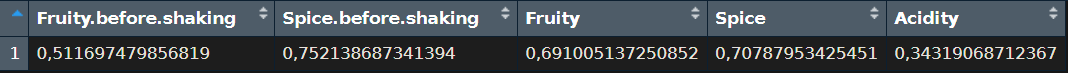
\includegraphics[scale=0.4]{images/R2_regression_Eq1.png}%
	}%
	\hfill%
	\subfloat[R2 de regression de l'équation 1]{%
		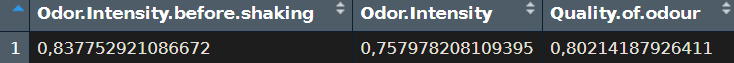
\includegraphics[scale=0.4]{images/R2_regression_Eq2.png}%
	}%
	\caption{R2 de regression linéaire des thèmes Odeur et Goût}
\end{figure}

On peut constater pour la régression (equation 1) des variables du thème \textit{Goût} sur les variables des thèmes \textit{Note_goût,~Plante,~Composition} sont relativement bonnes hormis pour la regression des variables \textit{Fruity.before.shaking} et notamment \textit{Acidity}. Si l'on représente les variable prédites avec celles mesurées on peut se rendre compte que les points sont assez bien répartis autour de la bissectrice mais que certains d'entre eux en sont également assez éloignés. En particulier on observe certains points extrèmes et des points assez éloignés de la bissectrice pour les deux variables \textit{Fruity.before.shaking,~Acidity} : 

\begin{figure}[htp] 
	\centering
	\subfloat[Regression de Fruity.before.shaking, équation 1]{%
		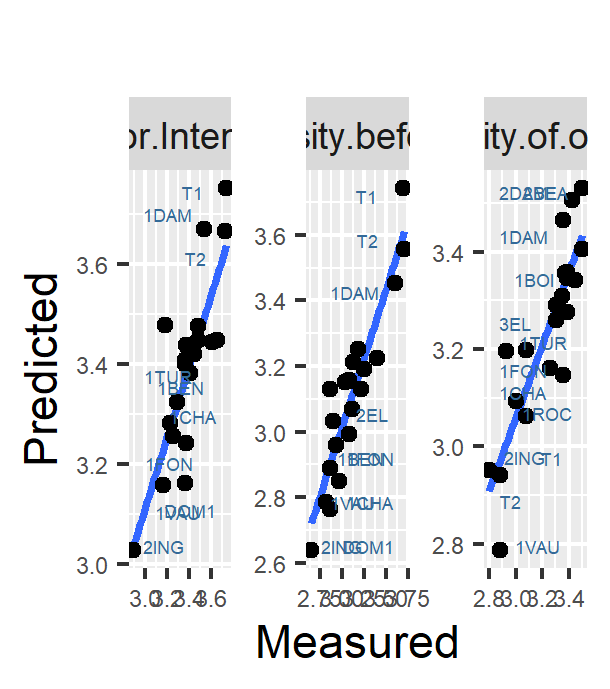
\includegraphics[scale=0.4]{images/Plot.Predictions_Eq (1).png}%
	}%
	\hfill%
	\subfloat[Regression de Spice.before.shaking, équation 1]{%
		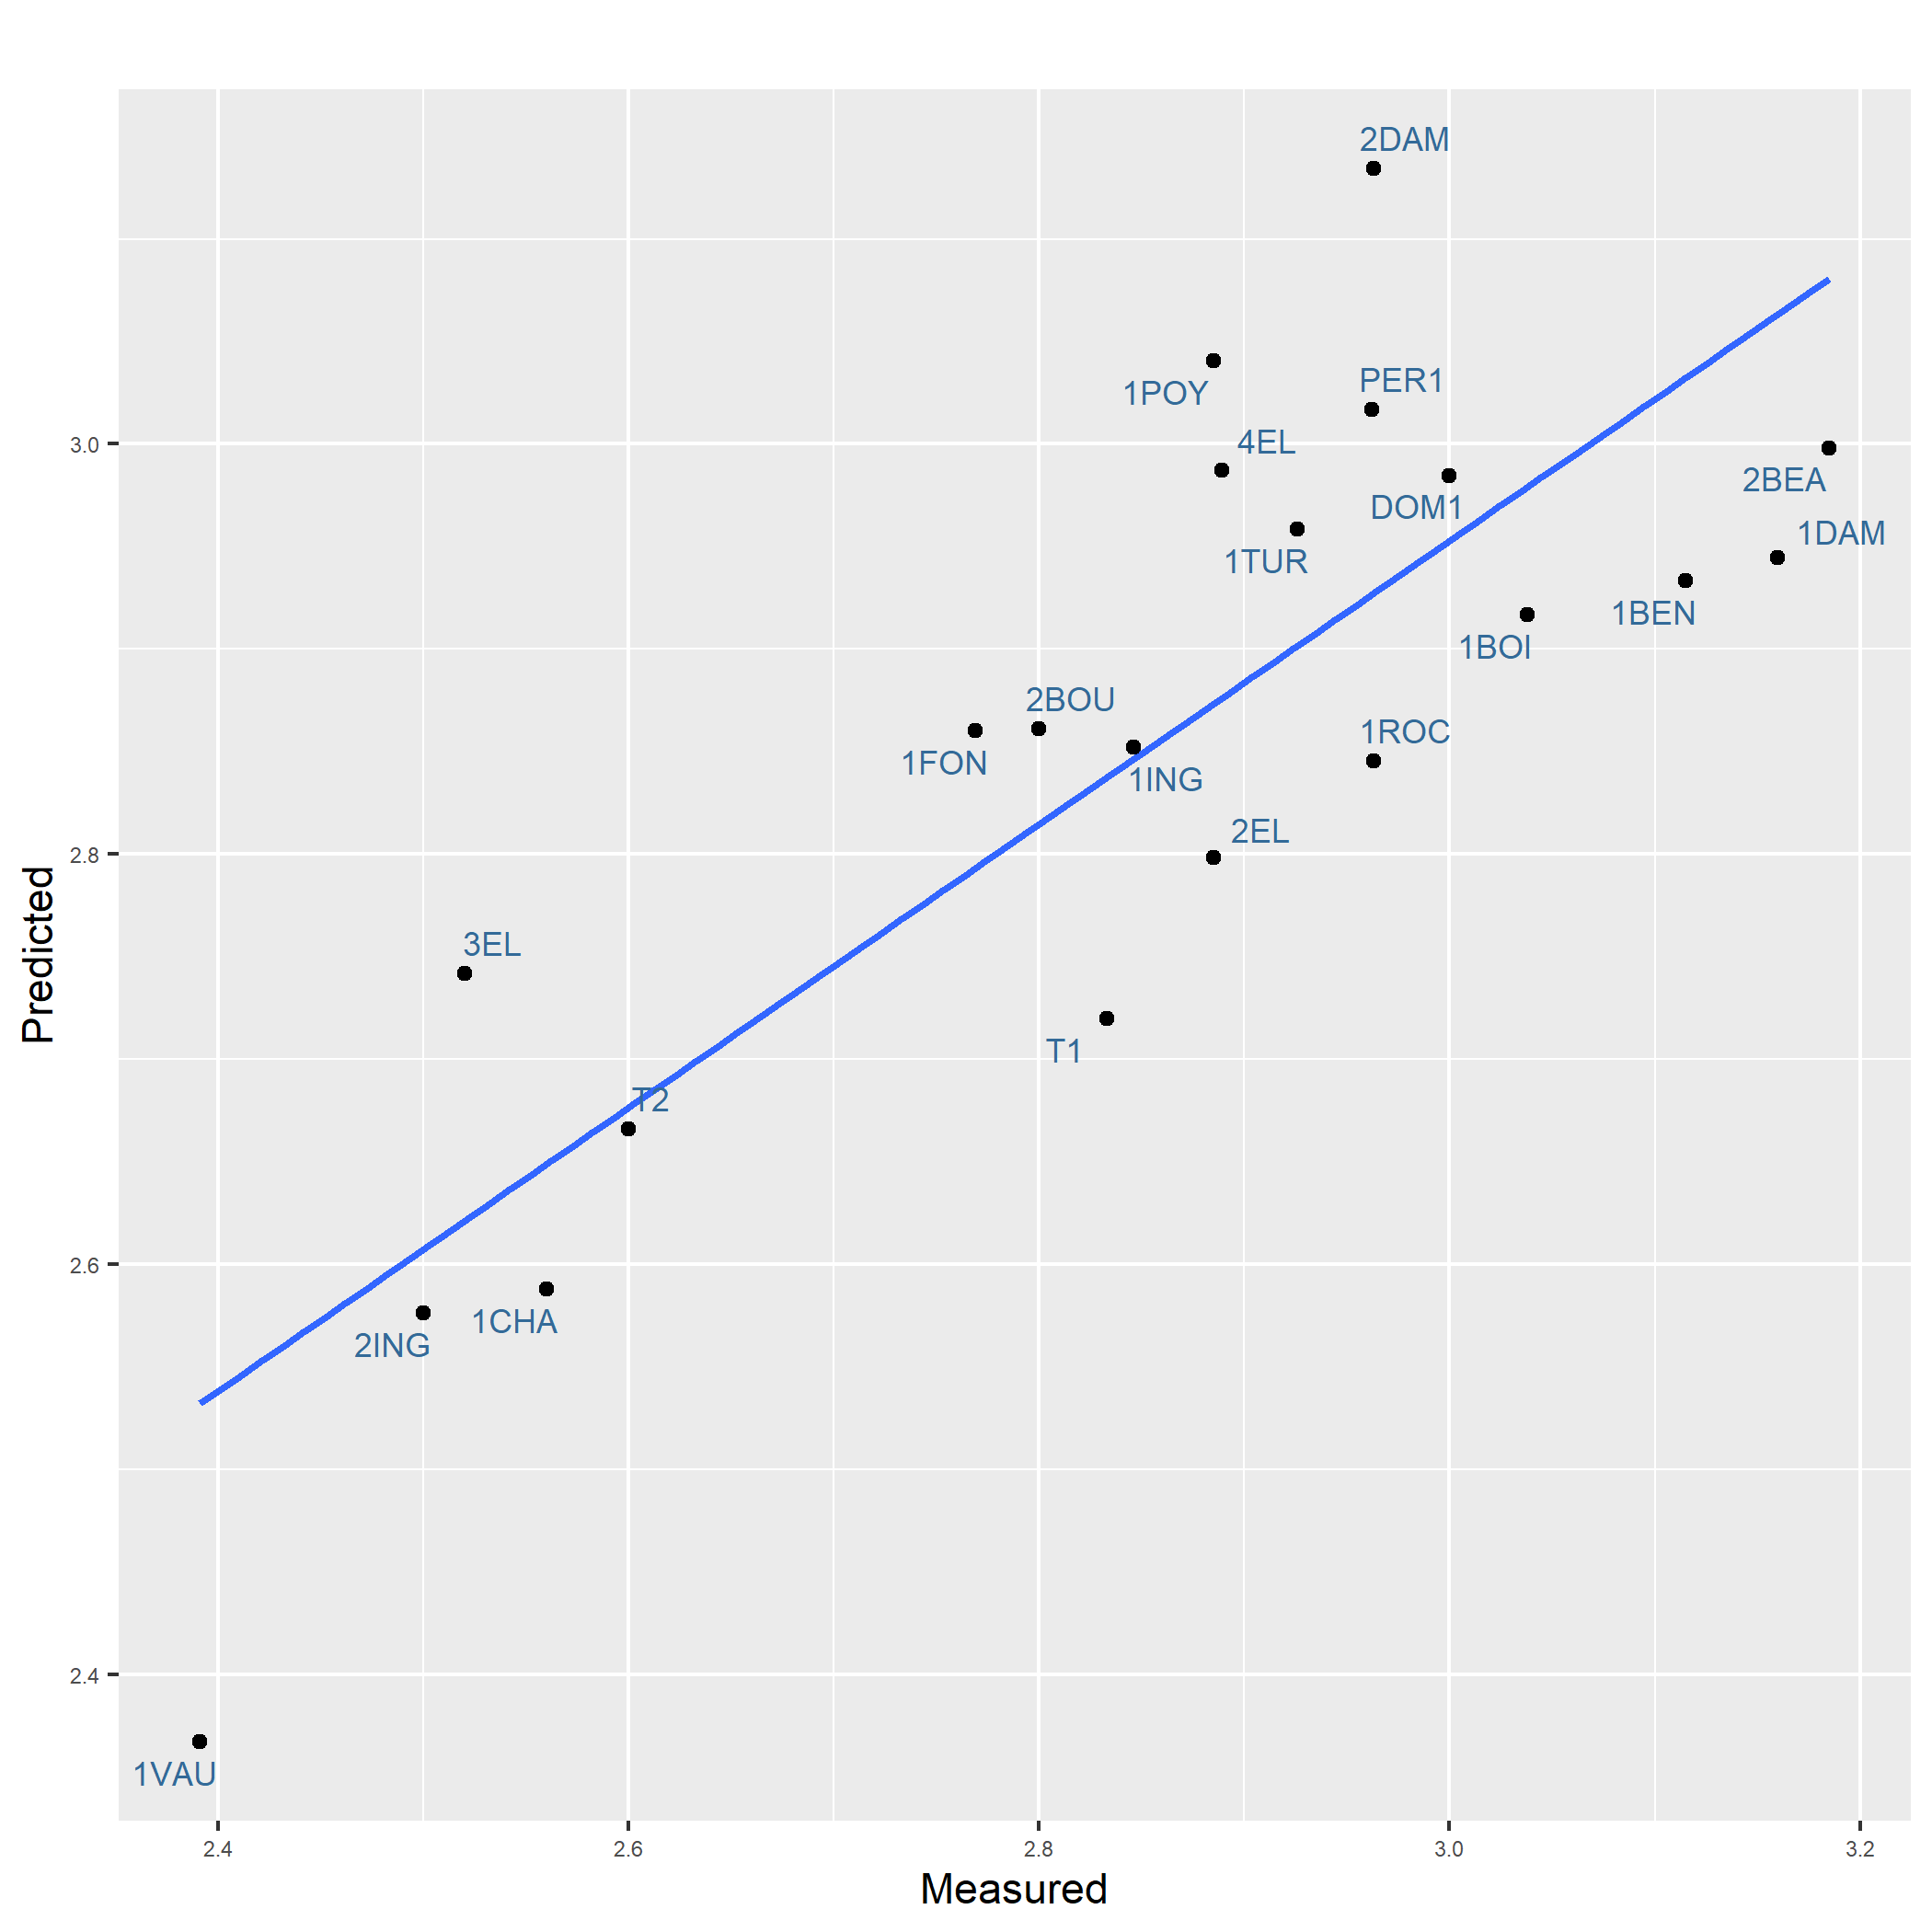
\includegraphics[scale=0.4]{images/Plot.Predictions_Eq (2).png}%
	}%
	\hfill%
	\subfloat[Regression de Fruity, équation 1]{%
		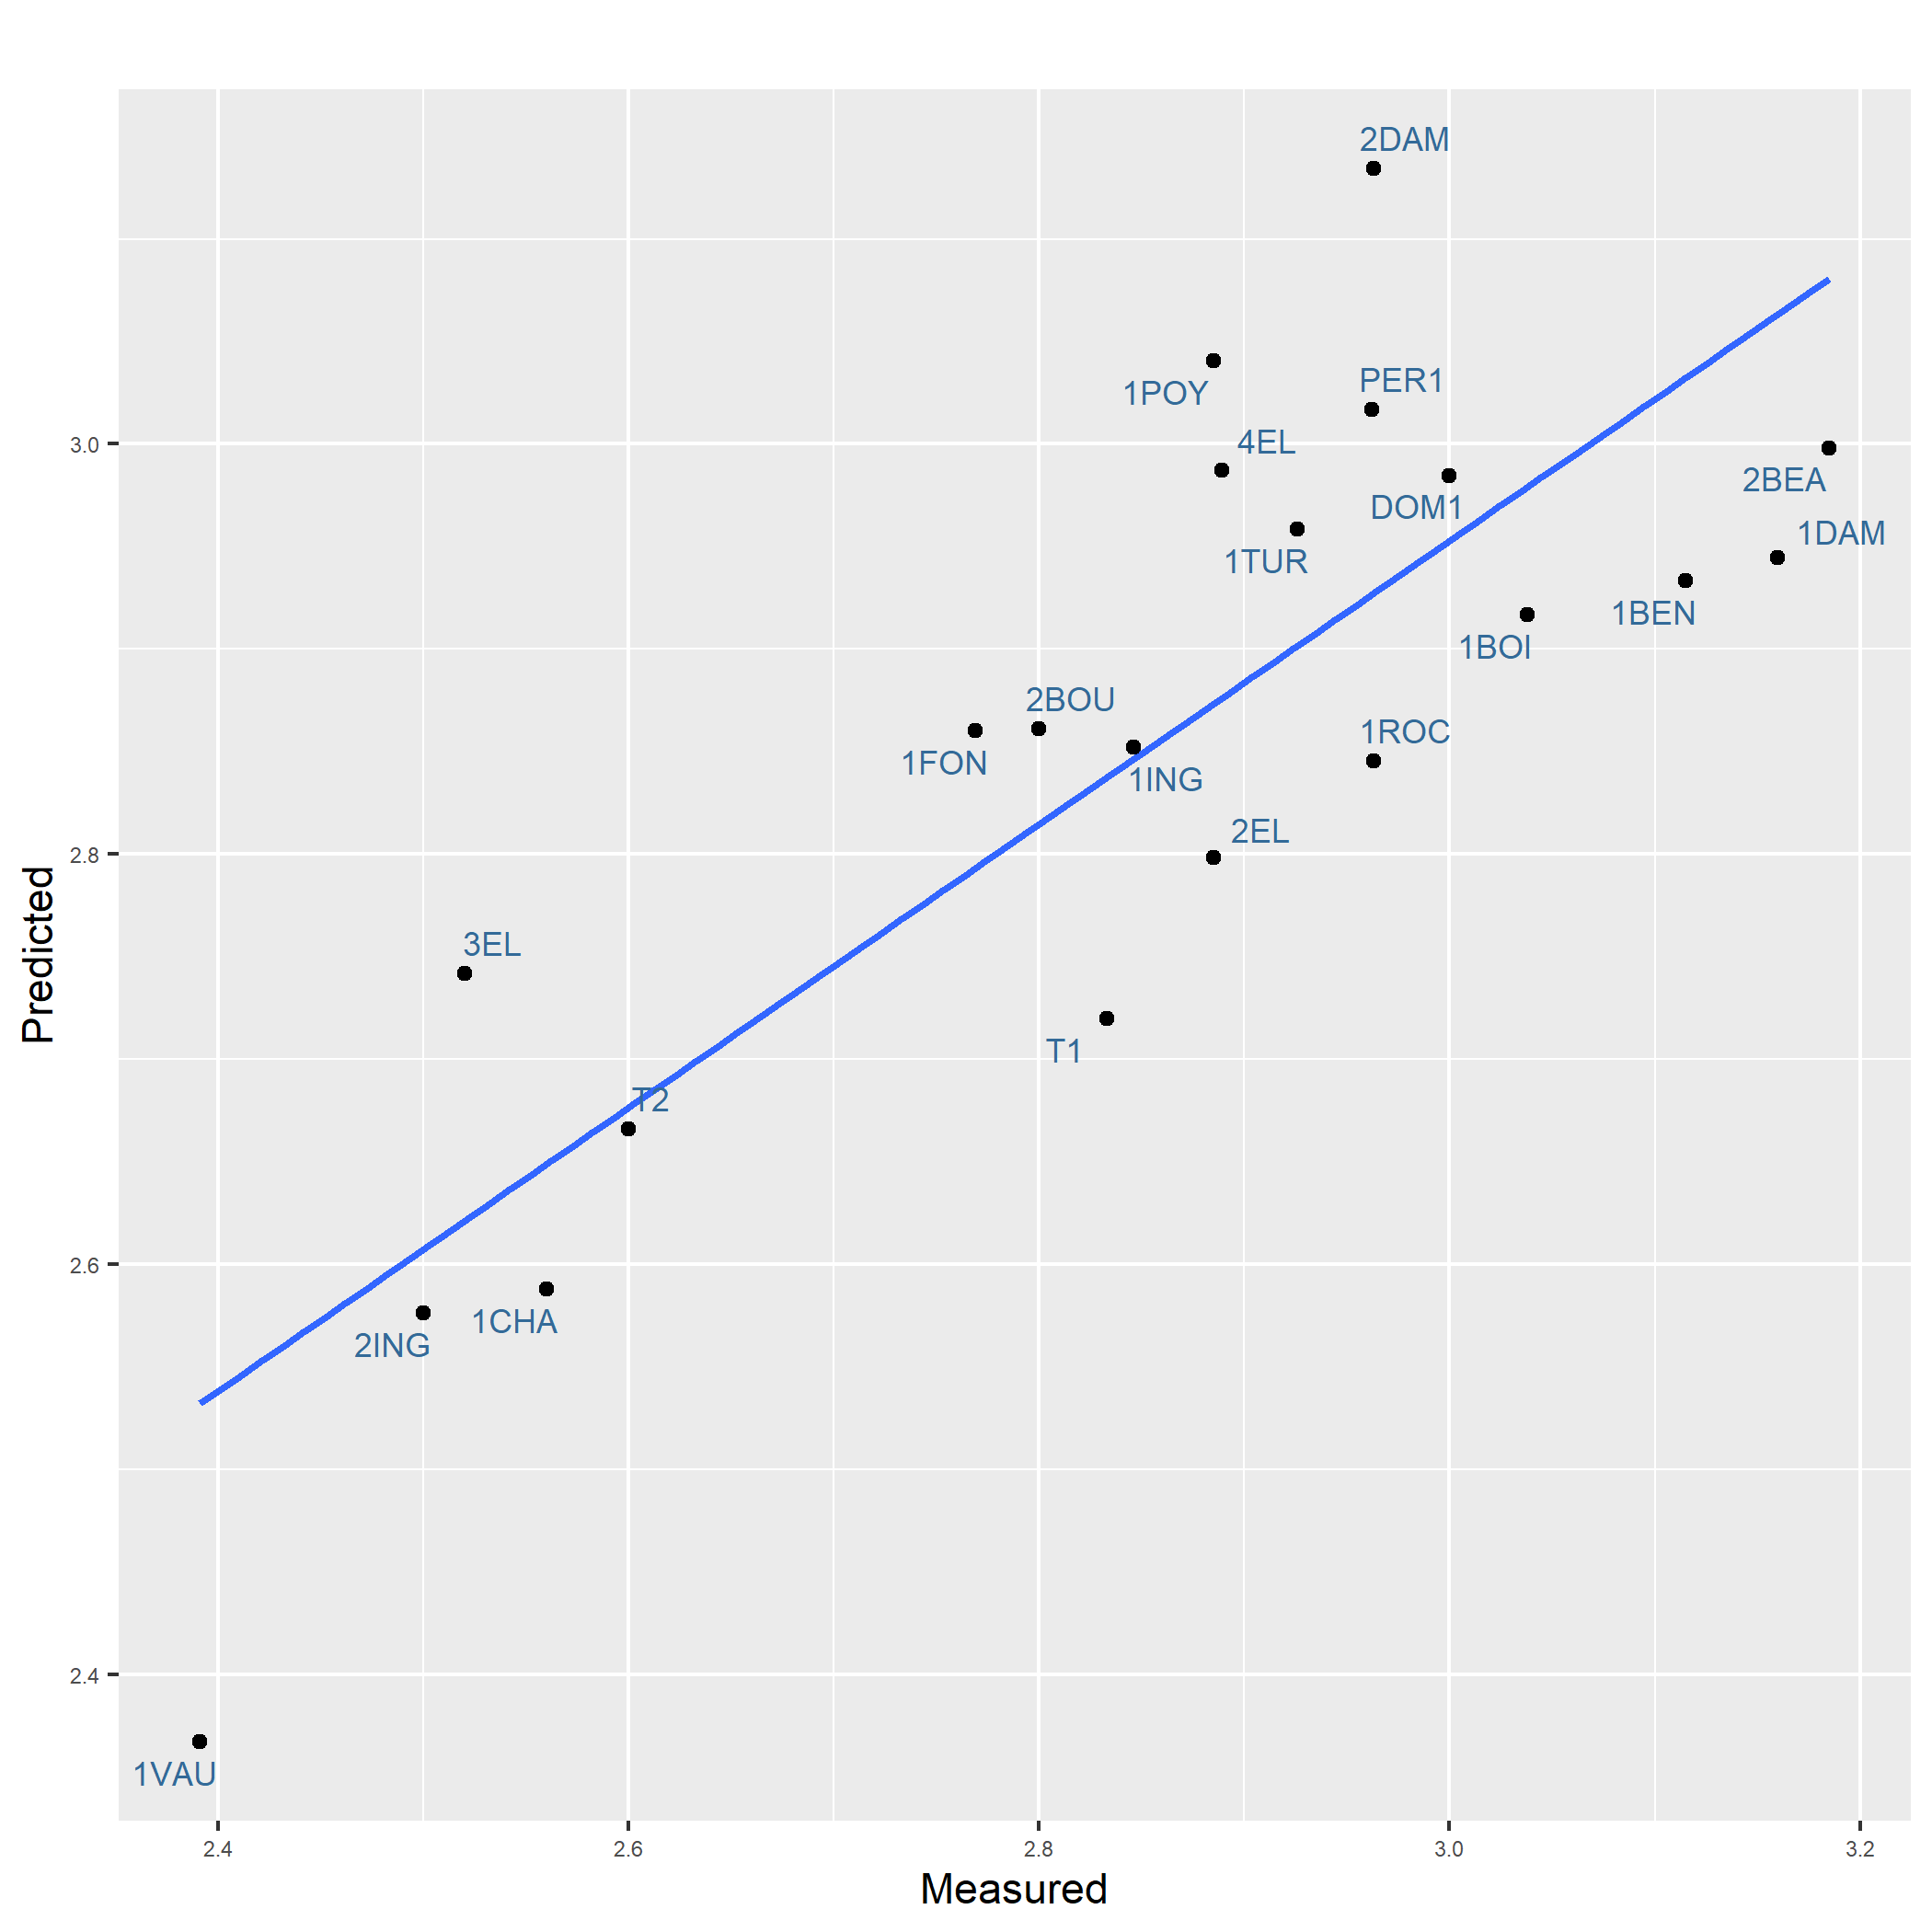
\includegraphics[scale=0.4]{images/Plot.Predictions_Eq (2).png}%
	}%
	\hfill%
	\subfloat[Regression de Spice, équation 1]{%
		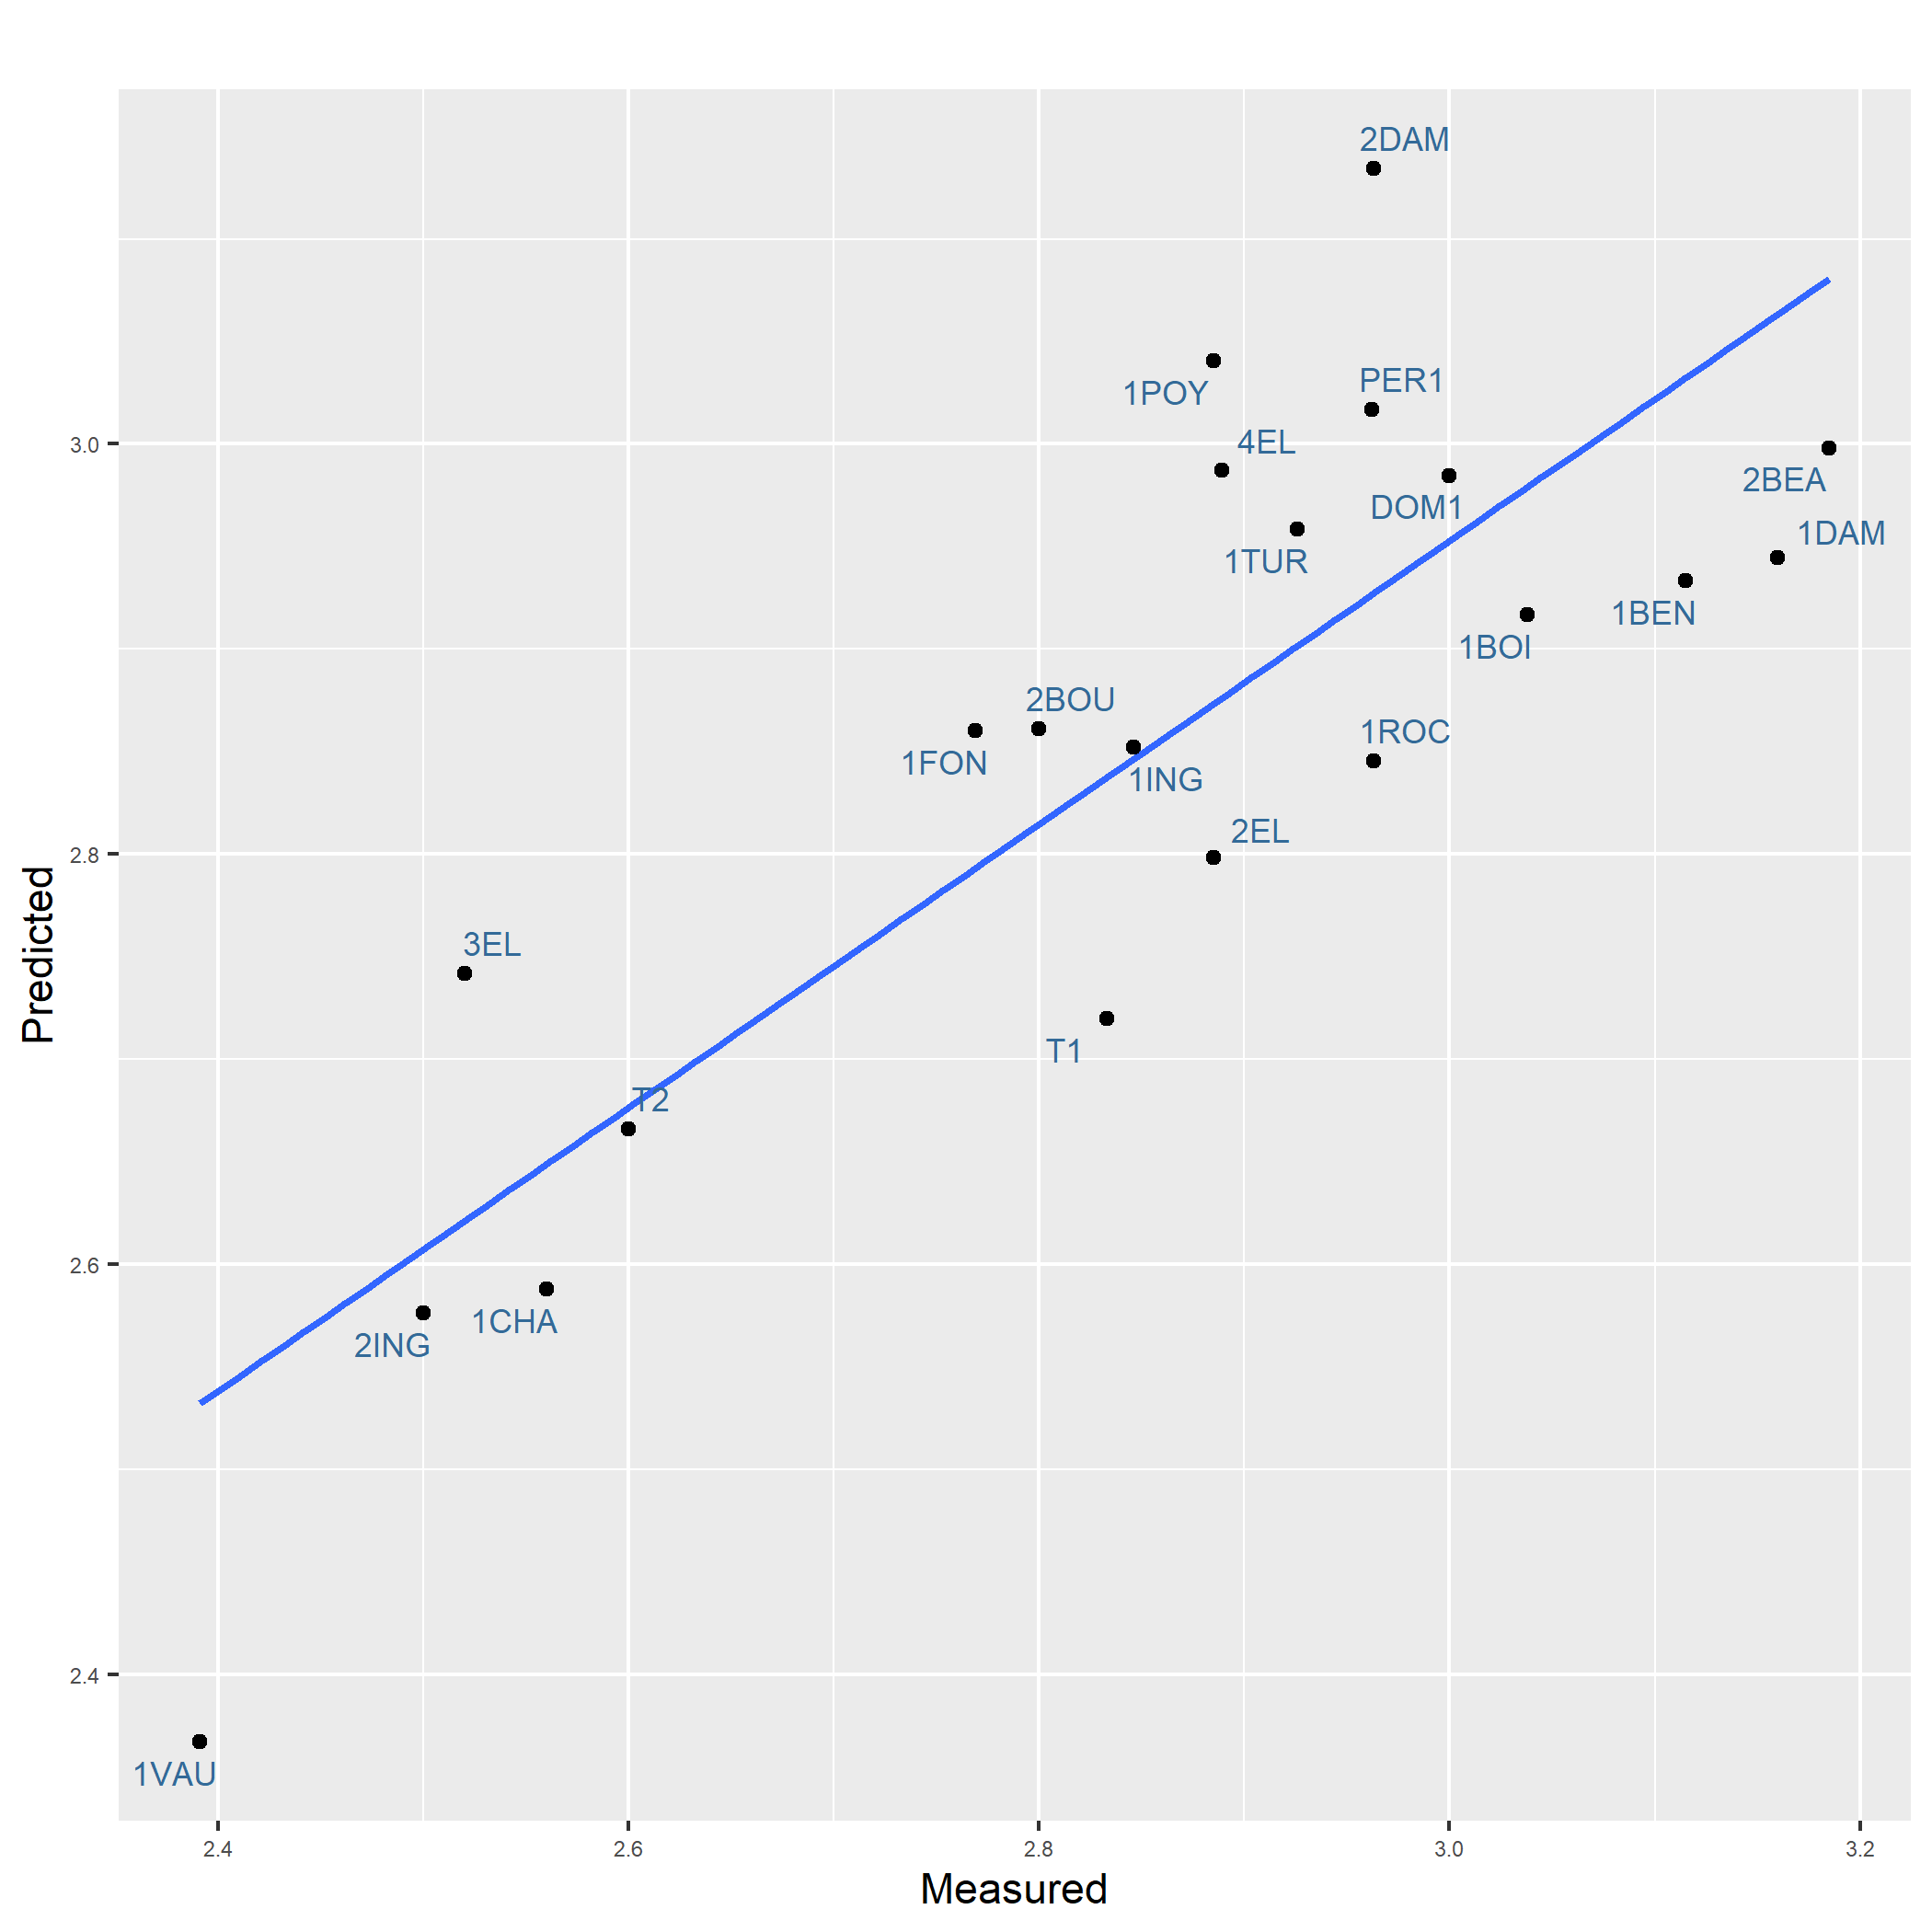
\includegraphics[scale=0.4]{images/Plot.Predictions_Eq (2).png}%
	}%
	\hfill%
	\subfloat[Regression de Acidity, équation 1]{%
		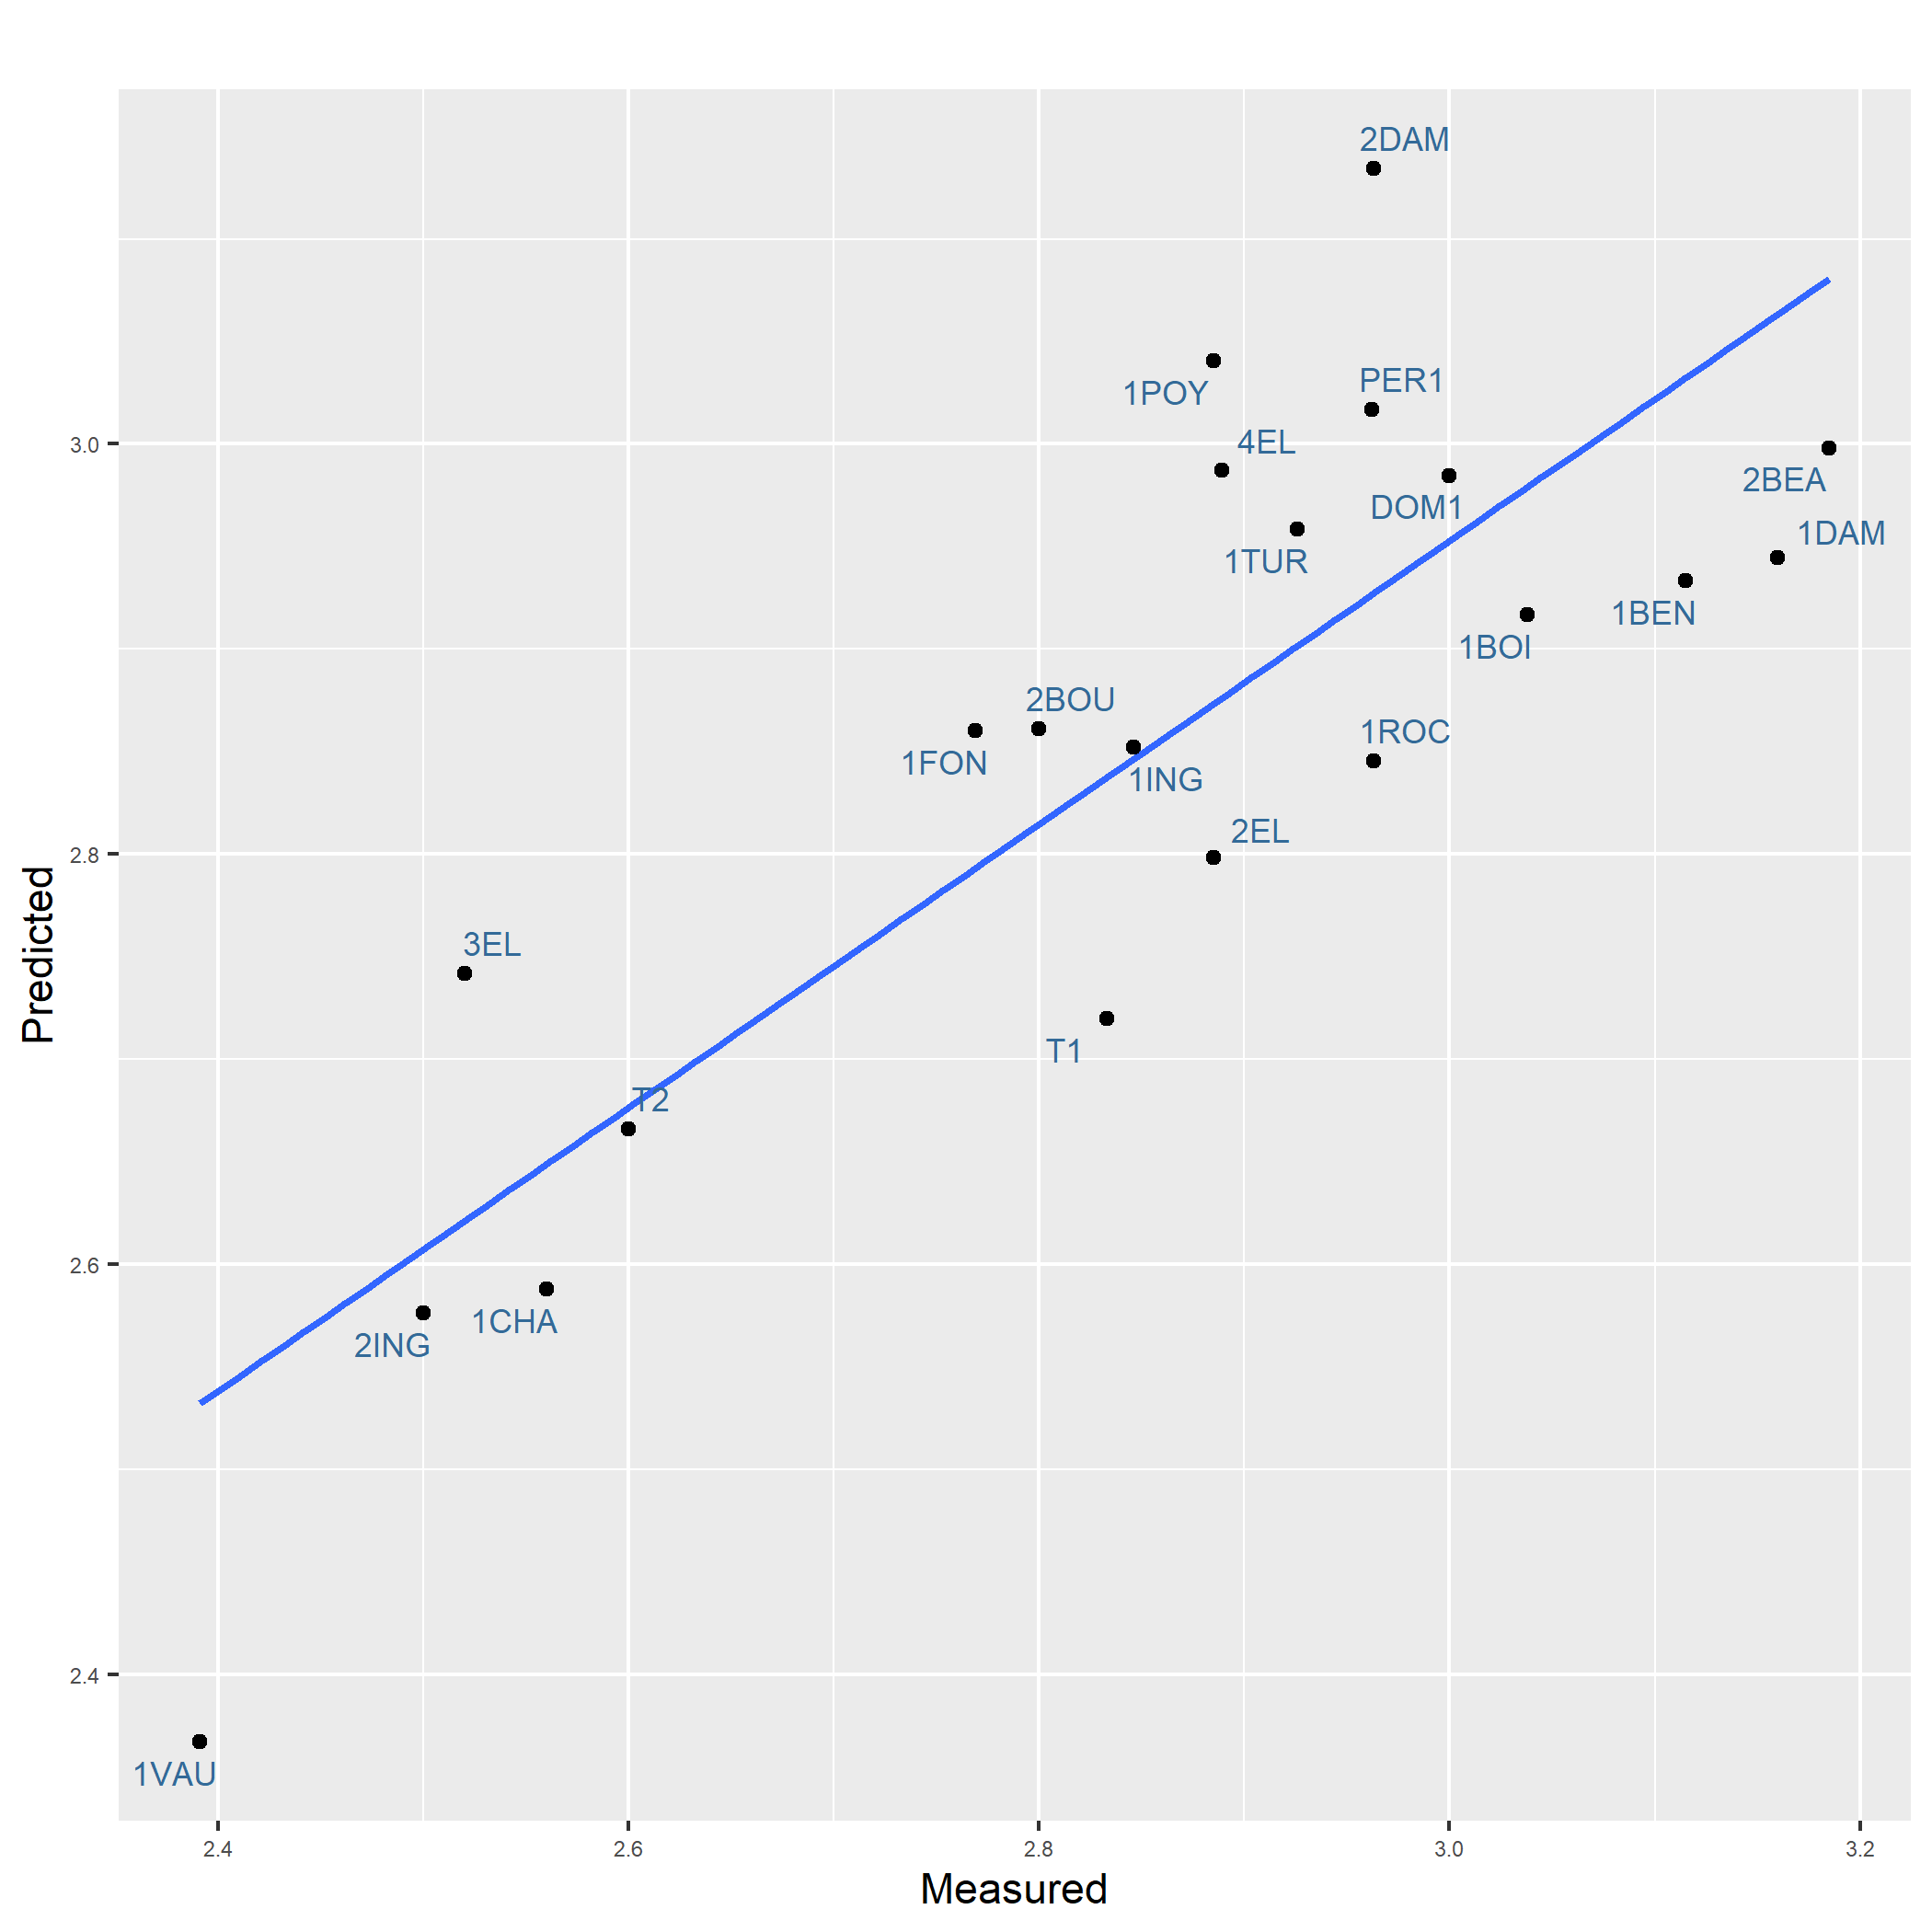
\includegraphics[scale=0.4]{images/Plot.Predictions_Eq (2).png}%
	}%
	\caption{Regression linéaire des variables \textit{Goût}, équation 1}
\end{figure}

On peut également se pencher sur la part que les variables jouent dans la prédiction des deux équations, nous permettant de déterminer les variables les plus pertinentes dans l'analyse des deux thèmes : 

\begin{figure}[htp] 
	\centering
	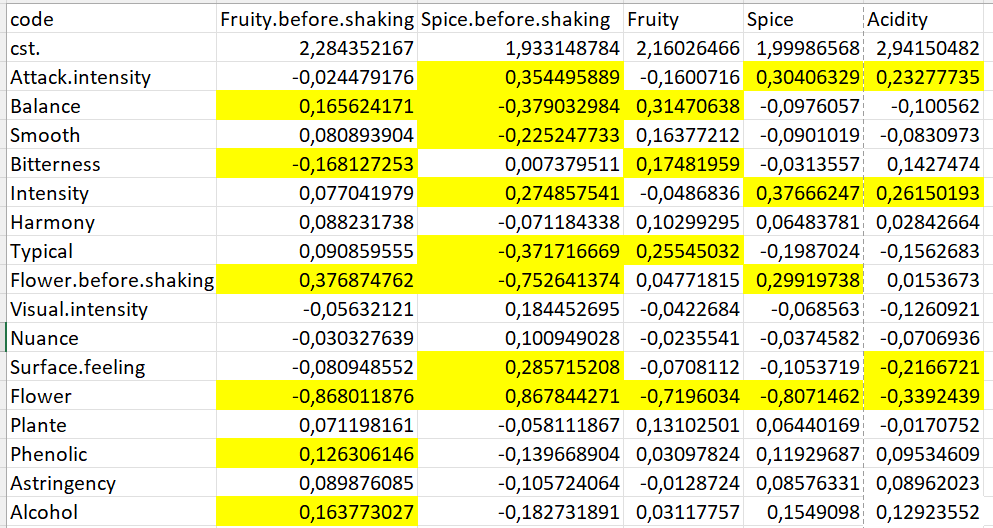
\includegraphics[scale=0.45]{images/Coeff_var_Eq1.png}
	\caption{Coefficients de régression linéaire des variables explicatives, équation 1}
\end{figure}


%interprétations

A présent, nous pouvons demander dans quelles dimensions les variables telles que ... sont-elles les plus liées : 

Pour le thème \textit{Odeur} : 
...
%interprétations



Dans cette sous-section, nous allons effectuer les mêmes démarches d'analyse que pour la sous-section précédante en effectuant desormais une \textit{Cross-validation backward} en partant du même modèle, ce qui enlève des composantes au fur et à mesure en testant quelle est l’erreur de prédiction pour chaque modèle testé. Nous pouvons ainsi déterminer le meilleur des ces modèles : 

%interprétations

\newpage



\section{Annexes}
%Ci dessous, l'export de code permettant d'afficher la liste des diviseurs de $464280$.
%\lstinputlisting[language=R, firstline=19, lastline=26]{code/script_projet_VE_COME_NIASSE.R}

\newpage

\section{Bibliographie}

\renewcommand\refname{}
\begin{thebibliography}{9}
	\bibitem{golfLion}
	\url{https://reporterre.net/Le-golfe-du-Lion-est-tres-vulnerable-a-la-montee-des-eaux}
	page web rédigée par Alexandre Brun et Benoît Devillers
	\bibitem{EM_algorithm}
	Frédéric Santos (2015). L'algorithme EM : une courte présentation
	\url{https://members.loria.fr/moberger/Enseignement/AVR/Exposes/algo-em.pdf}
\end{thebibliography}

\end{document}
